\chapter{Samarbejdsaftale}
Dokumentet her vil indeholde en beskrivelse over de overordnet aftaler som er relevant for gruppens arbejdsproces. Disse aftaler er blevet brugt for at opnå afklaring i forhold til forløbet og samtidig undgå misforståelser, som kan dukke op undervejs i processen.


\subsection{Kommunikation}
Kommunikation i gruppen til det fagrelevante forgår primært via slack og derudover bliver facebook også benyttet til de hurtige samtaler.

\subsection{Møder}
Der er blevet benyttet to forskellige former for møder, den ene er gruppemøder og den anden er vejledermøder. Gruppemøder har vi løbende, da vi mødes ind på skolen 3 gange om ugen og arbejder sammen (se figur 1.1). Somregel tager vi den interne møde omkring hvor langt man er i processen og de forhindringer der nu har været om onsdagen. Derudover er der ugentligt møde med vejlederen. Inden hver vejlermøde bliver der lavet en agenda over projektets status og de spørgsmål der nu er i gruppen. 

Processen for de to møde former bliver beskrevet nedenfor:
\begin{itemize}
    \item Giver besked via slack eller facebook hvis man ikke kan komme til møde
    \item Gruppemøder bliver holdt mindst en gange om ugen.
    \item Vejlermøde afholdes ugentligt.
    \item Forventes at agendaen/dagsorden gennemlæses af gruppens medlemmer og alle er forberedt til mødet.
    \item Under hver vejledermøde bliver der taget referet af mødet, hvor en af gruppens medlemmer tager ansvaret som referent.
  
\end{itemize}


    \begin{figure}[ht]
        \centering
    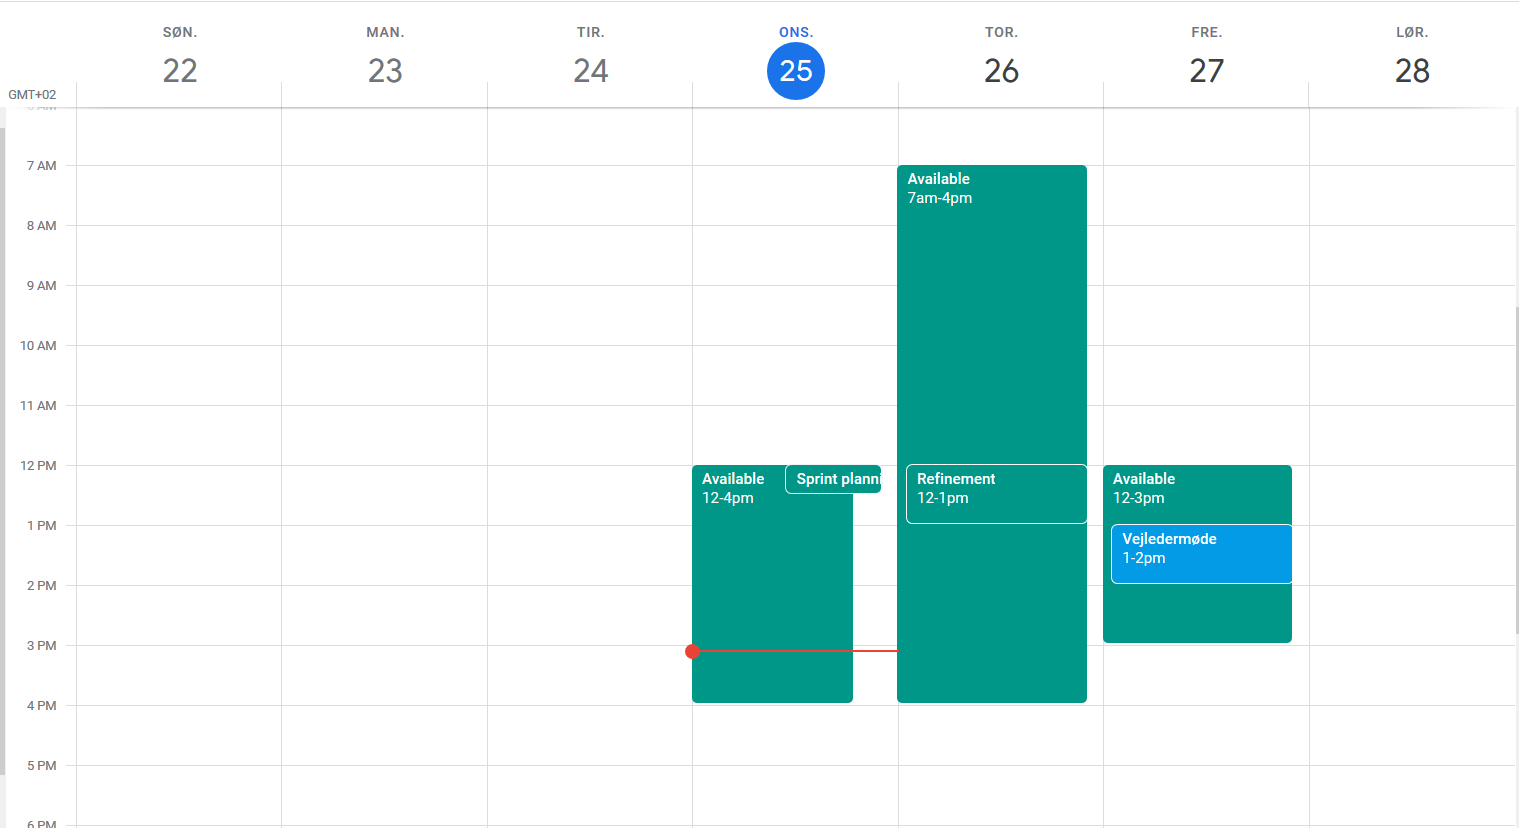
\includegraphics[width=0.8\textwidth]{Billeder/groupmeeting.png}
    \caption{Viser de dage vi arbejder på skolen.}
    \label{fig:figure2}
\end{figure}

\subsection{Værktøjer}
Dette afsnit vil indeholde beskrivelse og oversigt over de værktøjer der er aftalt at benytte i projektet.

\begin{itemize}
    \item \underline{\textbf{Zenhub}} benyttes til styring af Scrum.
    \item \underline{\textbf{GitHub}} er en hosting service, der ved hjælp af Git gør det muligt at bruge det til versionsstyring. de typer af dokumenter der bliver styret af Git er:
    \begin{itemize}
		\item Kode (sourcekode)
		\item LaTeX-dokumenter
		\item Back-end api'er
	\end{itemize} 
    \item \underline{\textbf{ Git}} distribueret versionsstyringssystem, som gør det muligt at vedligeholde kildekode. 
    \item \underline{\textbf{LaTex}} Dette bruges til at skrive alle tekst dokumenter.
    \item \underline{\textbf{elasticsearch}} bruges i forskellige cases, såsom:
    \begin{itemize}
       \item  Website søgning
       \item  Logning og loganalyse
       \item  Infrastrukturmetrics og containerovervågning
       \item  Overvågning af applikationens ydeevne
       \item Geospatial data analysis and visualization
       \item Sikkerhedsanalyse
       \item Forretningsanalyse
        
    \end{itemize}
   
    \item \underline{\textbf{ kubernetes}} benyttes til at administrere søgning efter tjenester og samtidig bruges den til justering af belastning, spore ressourceallokering, skalere ud fra udnyttelse af kapacitet og kontrollere individuelle ressourcers tilstand.
    \item \underline{\textbf{ ASP.NET}} bruges til at kode back-end.
    \item \underline{\textbf{ React}} til håndtering af front-end.
    \item \underline{\textbf{ Gitlab}} er en webbaseret DevOps livscyklusværktøj, som bruges til issues tracking og lave continuous ntegration (CI)/continuous delivery (CD) pipeline. 
    \item \underline{\textbf{ Gitbooks}} bruges til at gemme alle agendaer til vejledermøder, referet af møder, retrospectives og nogle værktøjer.
    \item \underline{\textbf{ Helm}} bruges til at hjælpe med at administrere Kubernetes-applikationer.
    \item \underline{\textbf{ .Net}} er et framework.
    \item \underline{\textbf{ Figma}} et værktøj der bliver brugt til at design af interface.
   
  
\end{itemize}


\subsection{Versionsstyring}
I projektet var der enighed om at Fagrelevant materiale vil blive administreret gennem GitHub. Herudover havde vi koblet gitlab til, så der kunne trackes issues og samtidig lave continuous ntegration (CI)/continuous delivery (CD) pipeline.



